\section{Durchführung}
\label{sec:Durchführung}
\begin{figure}
  \centering
  \begin{subfigure}{0.48\textwidth}
    \centering
    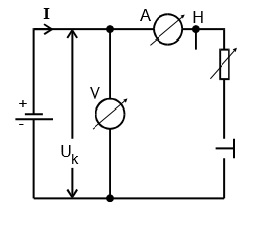
\includegraphics[height=5cm]{data/abb2.jpg}
    \caption{Messschschaltung zur Bestimmung von $U_0$ und $R_i$. \cite{V301}}
    \label{fig:abb2}
  \end{subfigure}
  \begin{subfigure}{0.48\textwidth}
    \centering
    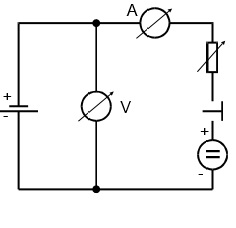
\includegraphics[height=5cm]{data/abb3.jpg}
    \caption{wie Abb.\ref{fig:abb2}, jedoch mit Verwendung einer Gegenspannung. \cite{V301}}
    \label{fig:abb3}
  \end{subfigure}
  \label{fig:Phasen}
\end{figure}
Es wird der Versuch entsprechend der Schaltbilder in Abb. \ref{fig:abb2} und Abb. \ref{fig:abb3} nacheinander aufgebaut.
Ein regelbarer Widerstand wird benutzt in den für die Versuchsteile nötigen Ohm-Bereichen.
Zuerst wird die Leerlaufspannung der Monozelle mit einem geeigneten Spannungsmesser ermittelt und der Eigenwiderstand $R_v$ notiert.
Für die erste Messreihe wird in Abb. \ref{fig:abb2} die Spannung $U_k$ in Abhängigkeit von I aufgetragen, für einen Belatungswiderstand von 0 bis 50 $\Omega$.
Danach wird an die Monozelle eine Gegenspannung, die ca. 2V größer als $U_0$ ist angelegt (siehe Abb. \ref{fig:abb3}).
Es wird ein Strom in umgekehrter Richtung fließen und die Klemmenspannung beträgt
\begin{equation}
  U_k = U_0 + \symbf{I} R_i
  \label{eqn:eq5}
\end{equation}
Es wird wieder $U_k$ in Abhängigkeit von $\symbf{I}$ gemessen.
Zuletzt wird die erste Messreihe wiederholt, nur nicht mit einer Monozelle, sondern dem Sinus- und Rechteckausgang eines RC-Generators.
\begin{itemize}
  \item Für die 1V-Rechteckspannung wird ein Variationsbereich von $R_a$: 20 - 250 $\Omega$ benutzt.
  \item Für die 1V-Sinusspannung wird ein Variationsbereich von $R_a$: 0.1 - 5 k$\Omega$ benutzt.
\end{itemize}
